\subsubsubsection{Probing the Higgs boson self-coupling in di-Higgs
  production with full $m_t$-dependence at NLO QCD}
\label{subsec:varylambda}

\begin{center}
\textit{by  Gudrun Heinrich, Stephen Jones, Matthias Kerner, Gionata Luisoni, Ludovic Scyboz}
\end{center}

While the couplings of the Higgs boson to vector bosons are very well measured meanwhile, 
and the couplings to third generation fermions also start to be well constrained and seem to confirm the Standard Model, 
the Higgs boson self-coupling could still reveal clear signs of New Physics. 
As it is not too far-fetched to have BSM scenarios in mind where the trilinear Higgs boson coupling $\lambda$ is different from the SM value at the ${\cal O}(10\%)$ level, while the deviations in other Higgs boson couplings are at the percent level, we consider $\lambda$ variations only in this section.
In particular, we announce a version of the {\tt ggHH} code~\cite{Borowka:2016ypz,Heinrich:2017kxx,Borowka:2016ehy} implemented in the {\tt POWHEG-BOX-V2}~\cite{Alioli:2010xd} where variations of  $\lambda$ are accessible to the user in a parton shower Monte Carlo program at full NLO.

\subsubsubsection{Total cross sections at different values of the trilinear coupling}

In Table \ref{tab:sigmatot} we list total cross sections at 14\,TeV and 27\,TeV for various values of the trilinear Higgs coupling $\lambda$. 
\begin{table}[htb]
\begin{center}
%\setlength{\extrarowheight}{3.0pt}
\begin{tabular}{| c | c | c |c|c|}
%\Xhline{2\arrayrulewidth}
\hline
&&&&\\
$\lambda_{\mathrm{BSM}}/\lambda_{\mathrm{SM}}$ & $\sigma_{\rm{NLO}}@14 \mathrm{TeV}$\,[fb] & $\sigma_{\rm{NLO}}@27 \mathrm{TeV}$\,[fb] &K-fac.@14TeV&K-fac.@27TeV\\
&&&&\\
\hline
1& 32.88$^{+13.5\%}_{-12.5\%}$&127.7$^{+11.5\%}_{-10.4\%}$ &1.66&1.62\\
\hline
2 & 14.91 &  59.10&&\\
\hline
2.4 & xx& yy&&\\
\hline
3& 19.82 & 69.84&&\\
\hline 
5 & 98.42& &&\\
\hline 
0 & 73.84& 275.29&&\\
\hline 
-1 & 137.69& &&\\
\hline
%\Xhline{2\arrayrulewidth}
\end{tabular}
\end{center}
\caption{Total cross sections for Higgs boson pair production at full NLO. The given uncertainties are scale uncertainties. 
A statistical uncertainty of about 0.3\% is not included in the quoted uncertainties.\label{tab:sigmatot}}
\end{table}
The results have been obtained using the parton distribution functions PDF4LHC15\_nlo\_100\_pdfas~\cite{Butterworth:2015oua,CT14,MMHT14,NNPDF},
along with the corresponding value for $\alpha_s$ for both the NLO and
the LO calculation.
The masses have been set to $m_h=125$\,GeV, $m_t=173$\,GeV,
and the top quark width has been set to zero. 
The scale uncertainties are the result of a 7-point scale variation around the central scale $\mu_0 = m_{hh}/2$,
with $\mu_{R,F}=c_{R,F}\,\mu_0$, where 
$c_R,c_F\in \{2,1,0.5\}$, except that the extreme variations $(c_R,c_F)=(2,0.5)$ and $(c_R,c_F)=(0.5,2)$
are omitted. 

Table~\ref{tab:sigmatot} also shows that the K-factors do vary substantially as functions of the trilinear coupling.
This fact is illustrated in Fig.~\ref{fig:Kfacvariation}, where it is demonstrated that the K-factor takes values between 1.57 and 2.16
if the trilinear coupling is varied between $-5\leq \chhh\leq 12$.

\begin{figure}[htb]
  \centering
    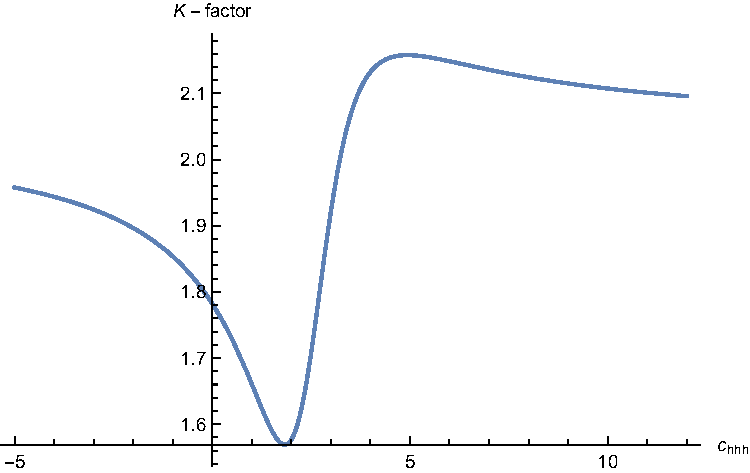
\includegraphics[width=0.4\textwidth]{\main/section3/plots/Kfac_varlambda.pdf}
%  \includegraphics[width=\textwidth]{plots/}
%    \caption{\label{fig:lambda_large_27}}
\caption{Variation of the NLO K-factor with the trilinear coupling, $\sqrt{s}=14$\,TeV.}
\label{fig:Kfacvariation}
\end{figure}


\subsubsubsection{Differential cross sections  at 14 TeV and 27 TeV}

In Figs.~\ref{fig:lambda_small} and ~\ref{fig:lambda_large} we show the $\mhh$ distribution for various values of $\chhh=\lambda_{\mathrm{BSM}}/\lambda_{\mathrm{SM}}$. 
The ratio plots show the differential K-factors. 

\begin{figure}[htb]
  \centering
  \subfloat[]{\label{fig:lambda_small_14}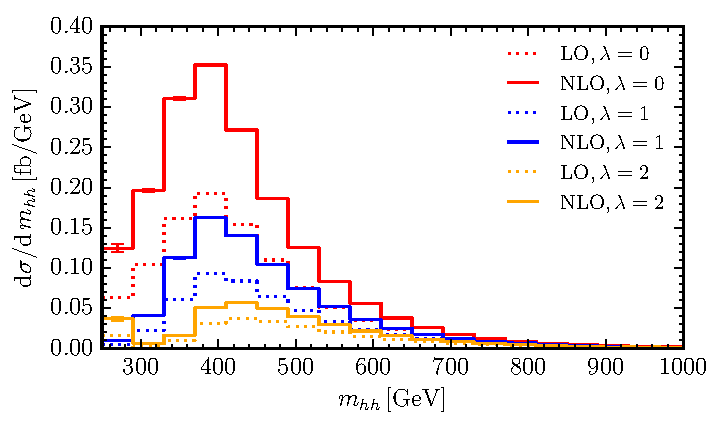
\includegraphics[width=0.6\textwidth]{\main/section3/plots/mhh_Kfac_14TeV_varylambda_small.pdf}}
  %\hfill
  %\subfloat[]{\label{fig:lambda_small_27}}
  %  \includegraphics[width=\textwidth]{plots/}
 \caption{Higgs boson pair invariant mass distributions for various values of $\lambda$ (relative to $\lambda_{\mathrm{SM}}$)  at 14\,TeV.}
\label{fig:lambda_small}
\end{figure}
%
\begin{figure}[htb]
  \centering
    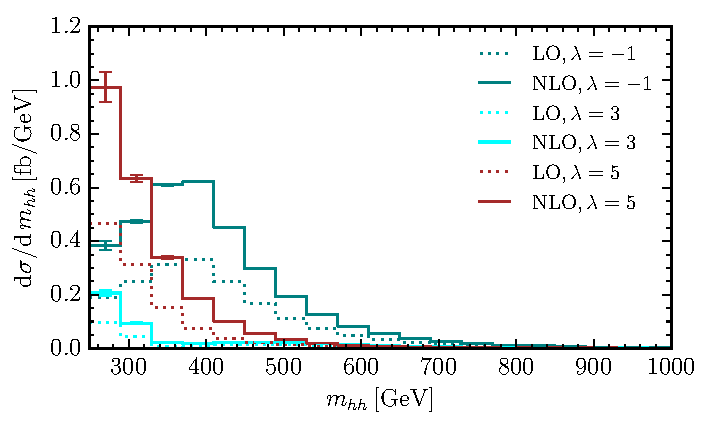
\includegraphics[width=0.6\textwidth]{\main/section3/plots/mhh_Kfac_14TeV_varylambda_large.pdf}
%  \includegraphics[width=\textwidth]{plots/}
%    \caption{\label{fig:lambda_large_27}}
\caption{Higgs boson pair invariant mass distributions for $\lambda/\lambda_{\mathrm{SM}}=-1,3,5$)  at 14\,TeV.}
\label{fig:lambda_large}
\end{figure}

{\it \ldots add 27TeV plots including ratio plots, to be completed}

\begin{figure}[ht]
\begin{center}
  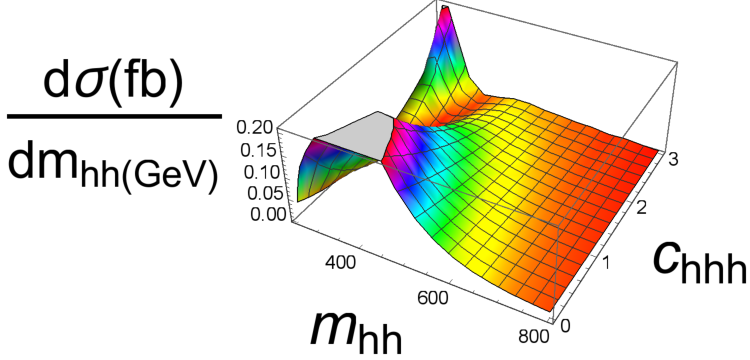
\includegraphics[width=0.45\textwidth]{\main/section3/plots/3D_mhh_chhh.pdf}    
\end{center}
\caption{3-dimensional visualisation of the $\mhh$ distribution at
  14\,TeV, as a function  $\chhh$.}
\label{fig:chhh_3D}
\end{figure}
Fig.~\ref{fig:chhh_3D} shows the Higgs boson pair invariant mass
distributions at NLO as a function of $\chhh$  as 3-dimensional heat maps.
The other couplings are fixed to their SM values.
 
%\bibliography{bib/refs_HH_lambda}


